\begin{figure*}[ht]
\centering
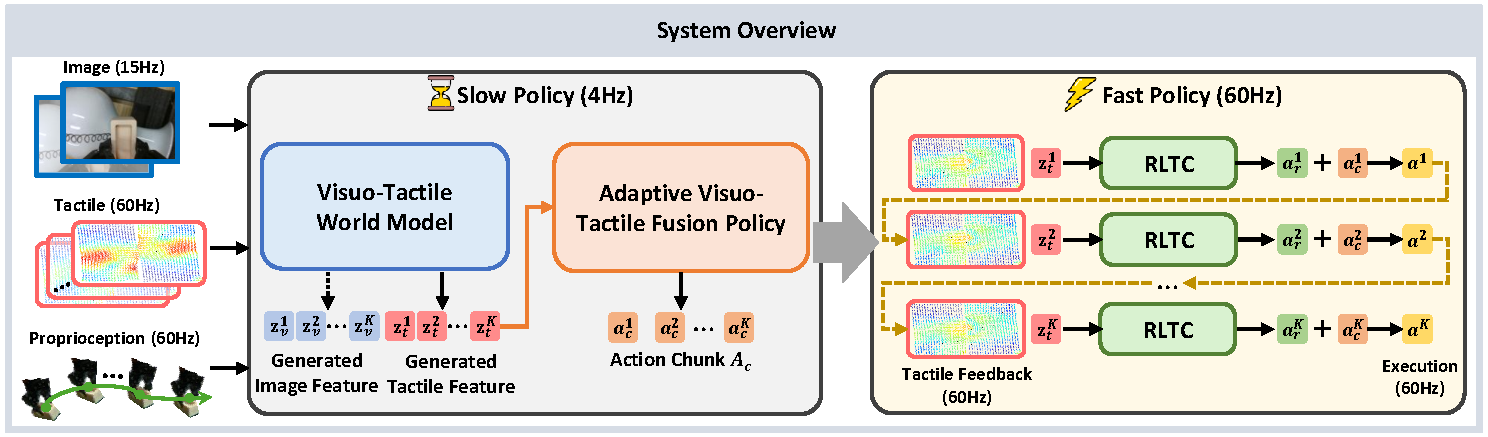
\includegraphics[width=0.95\linewidth]{fig/system.pdf}
\caption{\textbf{{System Overview}}. OmniVTA is a hierarchical slow–fast policy for contact-rich manipulation. The slow policy contains a visuo-tactile world model and an adaptive fusion policy to generate long-horizon action chunks from multi-modal inputs. 
The fast policy outputs high-frequency refinements at $60$~Hz using tactile feedback. 
Final actions are a weighted summation of slow-planned and fast-refined outputs, enabling both long-horizon planning and reactive control for robust manipulation.}
\label{fig:system}
\end{figure*}

\section{Methodology}



\subsection{System Overview}
To achieve stable and robust contact-rich manipulation, we introduce {OmniVTA}, a hierarchical slow-fast manipulation policy built upon a visuo-tactile world model, as illustrated in Fig.~\ref{fig:system}. OmniVTA explicitly decomposes manipulation into \emph{slow planning} and \emph{fast reflexive control}. 
The \emph{Slow Policy} integrates the Visuo-Tactile World Model (VTWM) and the Adaptive Visuo-Tactile Fusion Policy (AFP) to perform long-horizon action chunk planning from low-frequency visual observations, high-frequency tactile signals, and proprioceptive states. To improve efficiency, the world model predicts future tactile signals without generating visual observations during inference, enabling higher-frequency rollout while preserving contact-relevant dynamics.
The \emph{Fast Policy} is implemented as a Reflexive Latent Tactile Controller (RLTC), inspired by the reflexive control paradigm~\cite{xu2025aprebot, xu2025rebot}, which outputs fine-grained corrective actions at 60~Hz based on both predicted and observed tactile signals. This controller refines the action sequences generated by the slow policy by combining the planned actions with the controller outputs through a weighted summation, where the controller contribution is scaled by a predefined coefficient before execution on the robot.
This slow-fast decomposition enables both long-horizon planning and high-frequency reflexive control, which are critical for contact-rich manipulation.

In the following, we detail the components of OmniVTA. Sec.~\ref{sec:tacvae} introduces the TactileVAE for tactile feature extraction. Sec.~\ref{sec:vtwm} presents the Visuo-Tactile World Model, which captures contact dynamics via joint visual-tactile prediction. Sec.~\ref{sec:fusion_policy} describes the adaptive fusion policy with a gated mechanism~\cite{cao2023multi} for integrating visual and tactile features. Sec.~\ref{sec:controller} details the Reflexive Latent Tactile Controller.



\subsection{TactileVAE}
\label{sec:tacvae}
TactileVAE aims to rapidly extract low-dimensional, continuous, and task-agnostic tactile representations for downstream prediction and policy learning. For optical tactile sensors, instead of using high-resolution tactile images, we adopt \textit{3D marker displacement} as tactile input. This representation captures contact-induced surface deformation while maintaining significantly lower resolution, enabling efficient feature extraction and higher-frequency inference. The structure of the TactileVAE is shown in Fig.~\ref{fig:vae}, which contains a spatial-temporal encoder and an implicit deformation decoder.

\subsubsection{Encoder}
We construct a spatio-temporal encoder to extract compact tactile token representations. Since the markers on the tactile surface are uniformly distributed, a single-frame tactile observation can be represented as a tensor of size $H \times W \times 3$ where $H$ and $W$ denote the number of markers along the $y$- and $x$-axes, respectively, and the channel dimension corresponds to the marker displacement along the $x$, $y$, and $z$ directions.

As tactile sensing typically operates at a higher frequency than vision, we perform joint temporal and spatial compression to reduce the number of tactile tokens and align them with visual tokens in time. To this end, we adopt a \textit{3D convolution-based variational autoencoder (VAE)} and pretrain it on a large corpus of real tactile data to learn low-dimensional, task-agnostic latent features.

As illustrated in Fig.~\ref{fig:vae}, the encoder consists of a projection-in layer (causal 3D convolution), $M$ downsampling modules, and a projection-out layer (causal 3D convolution). The input is encoded into a latent feature map of size $\frac{H}{s} \times \frac{W}{s} \times C$, where $s = 2^M$ is the spatial downsampling factor and $C$ is the latent dimension. We adopt \textit{causal 3D convolutions} along the temporal axis so that the latent representation at time $t$ depends only on current and past observations, ensuring consistency between training and real-time deployment.

\subsubsection{Decoder}

Instead of reconstructing pixels as in conventional VAEs, we employ an \textit{implicit neural representation (INR)}~\cite{sitzmann2020implicit} decoder to model a continuous tactile deformation field conditioned on spatial coordinates. Implicit representations are well-suited for modeling continuous signals and have been widely used in computer vision tasks such as geometric reconstruction~\cite{zhong20233d, park2019deepsdf} and dense prediction~\cite{chen2023dpf, yu2026infinidepth}. Since marker displacement arises from the continuous deformation of the elastomer surface under contact, we model the deformation field as a continuous function:

\begin{equation}
    \mathbf{d}(\mathbf{x}) = \mathcal{D}_{\theta} \left( \gamma(\mathbf{x}), \Phi(\mathbf{z}_{t}, \mathbf{x}) \right),
\end{equation}
where $\mathbf{x} \in \mathbb{R}^2$ denotes the spatial coordinate, $\mathbf{z}_{t}$ is the latent feature map, $\gamma(\cdot)$ represents positional encoding, $\Phi(\mathbf{z}_{t},\mathbf{x})$ retrieves local features from $\mathbf{z}_{t}$ via spatial interpolation, and $\mathcal{D}_{\theta}$ is an MLP decoder that predicts the 3D deformation $\mathbf{d}(\mathbf{x}) \in \mathbb{R}^3$. 
During training, we uniformly sample query points in the latent feature map and extract their local features, which, together with the corresponding positional encodings, are fed into the decoder to predict the corresponding \textit{3D deformation vector}. This yields a continuous reconstruction of the tactile surface deformation field.
% During training, we uniformly sample query points within the latent feature map and extract the corresponding local features. Together with the positional encoding of the query coordinates, these features are fed into the decoder to predict the corresponding \textit{3D deformation vector}, thereby reconstructing the continuous deformation field of the tactile surface.

\subsubsection{Training Loss}
For supervision, the ground-truth deformation $\hat{\mathbf{d}}(\mathbf{x})$ at each query point $\mathbf{x}$ is obtained by interpolating the original 3D deformation. 
The TactileVAE is trained with a reconstruction loss and a KL regularization term~\cite{kingma2013auto}:

\begin{equation}
\mathcal{L}_{\text{TacVAE}} 
= \|\mathbf{d}(\mathbf{x}) - \hat{\mathbf{d}}(\mathbf{x})\|_2^2
+ \lambda_{\mathrm{KL}} \, \mathcal{L}_{\mathrm{KL}}.
\end{equation}

\begin{figure}[t]
\centering
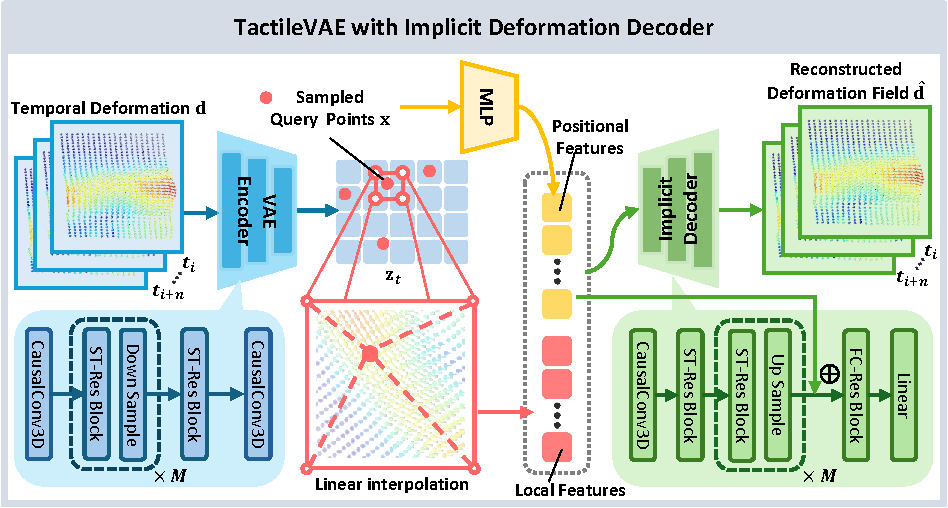
\includegraphics[width=\linewidth]{fig/vae.pdf}
\caption{\textbf{Overview of TactileVAE.} The model encodes 3D marker displacements into spatio-temporal features, and reconstructs the deformation via an implicit decoder that represents the deformation as a continuous field.}
\label{fig:vae}
\end{figure}


\begin{figure*}[ht]
\centering
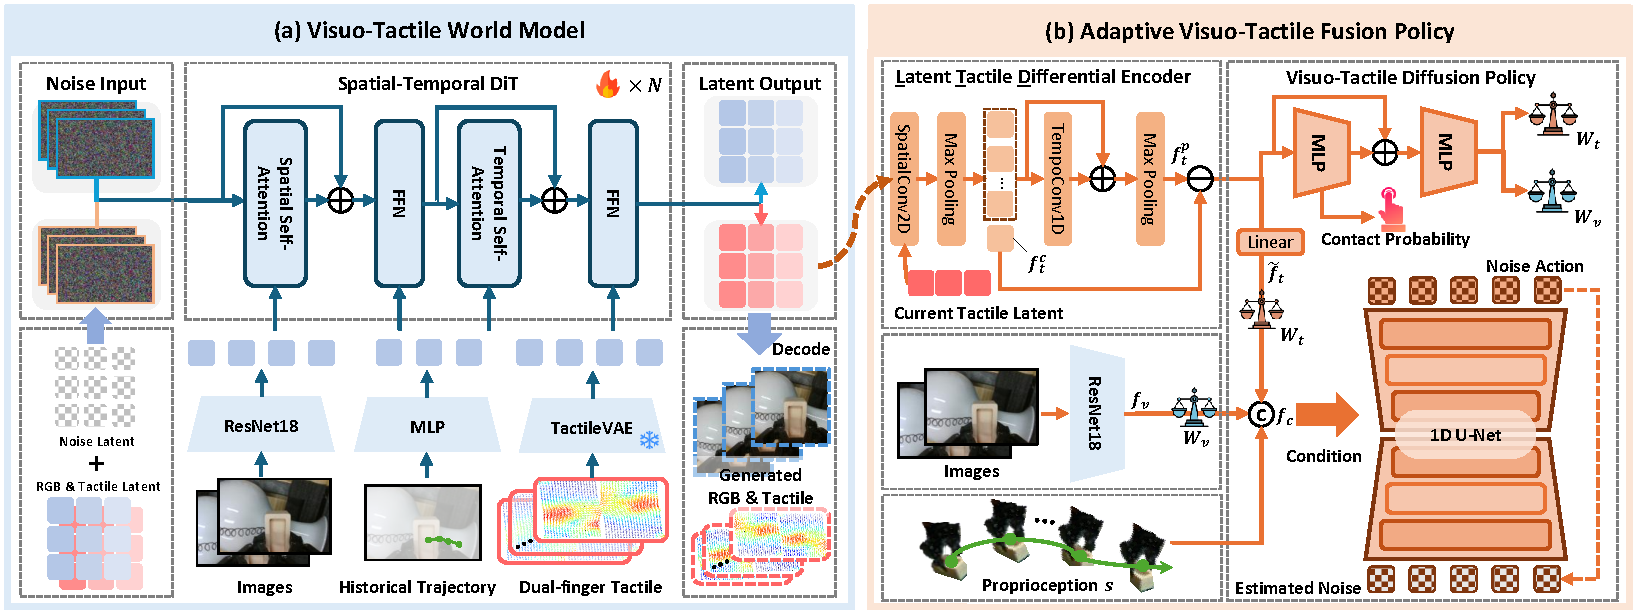
\includegraphics[width=0.95\linewidth]{fig/slow-policy.pdf}
\caption{\textbf{Overview of the Slow Policy.} \textbf{(a):} The proposed Visuo-Tactile World Model takes noisy tactile and visual latent sequences as input and jointly generates both modalities via a two-stream spatio-temporal diffusion transformer. \textbf{(b):} The Adaptive Visuo-Tactile Fusion Policy employs a Latent Tactile Differential Encoder to effectively encode the observed and predicted tactile and a gating mechanism to adaptively balance tactile and visual information for robust action planning.}
\label{fig:slow_policy}
\vspace{-5mm}
\end{figure*}

\vspace{-5mm}
\subsection{Visuo-Tactile World Model}
\label{sec:vtwm}
In this section, we present the Visuo-Tactile World Model, which adopts a two-stream conditional generative framework and explicitly models the temporal evolution of visual observations and tactile signals, thereby learning a dynamic prior for multimodal interactions. Overall, it consists of three key modules. The two-stream world model separately characterizes the dynamic generation process of the visual and tactile modalities while performing coordinated prediction under a shared condition. The multimodal observation conditioner jointly encodes vision, tactile, and actions, providing consistent conditioning for the generation process. The dynamic-aware weighted loss further emphasizes regions with high-frequency tactile variations and salient contact responses, improving the modeling of fine-grained tactile dynamics.

\subsubsection{Two-stream World Model}
To model the evolution of visual observations and tactile states during policy execution, we build a two-stream visuo-tactile world model, as shown in Fig.~\ref{fig:slow_policy} (a). Both branches employ a spatial-temporal diffusion transformer~\cite{peebles2023scalable}, which stacks transformer blocks along temporal and spatial axes. Specifically, the model takes the past $c$ frames as conditioning and iteratively denoises to generate multiple future frames, yielding a probabilistic model of future dynamics. The diffusion objective is defined as

\vspace{-2mm}
\begin{equation}
\mathcal{L}_{\text{diffusion}}=\mathbb{E}_{\mathbf{z}_o, \boldsymbol{\epsilon}, t}\left[\sum_{i=1}^K \left(1-m_i\right) \odot \left\|\epsilon_i-\boldsymbol{\epsilon}_\theta\left(\mathbf{z}_o, t\right)_i\right\|_2^2\right],
\end{equation}
where $\mathbf{z}_o = \left\{ \mathbf{z}_o^{1}, \dots, \mathbf{z}_o^{K} \right\}$ denotes a sequence of observation latents (including tactile latent $\mathbf{z}_t$ and visual latent $\mathbf{z}_v$), and $\boldsymbol{\epsilon}_\theta(\mathbf{z}_o, t)$ predicts the noise for the entire sequence. Each $\mathbf{z}_o^{i}$ corresponds to the encoded observation at timestep $i$. The mask $m$ provides temporal conditioning, encouraging the model to leverage historical observations for predicting future states.
At the modality encoding layer, the visual branch uses an SD-VAE~\cite{rombach2022high} to extract image latents, while the tactile branch employs the TactileVAE pretrained in the previous stage to compress tactile signals. After obtaining the latent representations of vision and touch, the two modalities are fed into their corresponding spatial-temporal diffusion models, enabling parallel modeling and joint generation. 

\subsubsection{Multi-modal Observation Conditioner}
To model joint visual-tactile dynamics effectively, we design a multi-modal conditional encoder for visual-tactile-action interactions. This module first performs feature extraction and temporal aggregation separately for visual observations, tactile embeddings, and action sequences, where each action is represented as the 2D image-plane projection of the 3D end-effector position. We observe that this representation improves robustness to variations in manipulation locations. The modalities are then fused in a shared linear projection space to produce a fixed-dimensional conditioning vector. This vector is injected as a shared prior into both the tactile and visual world models, aligning the two branches and improving cross-modal consistency during dynamic prediction.

\subsubsection{Dynamic-aware Weighted Loss}
To supervise high-frequency dynamic changes in tactile signals more effectively, we introduce a Dynamic-Aware Weighted Loss. Specifically, the loss constructs a dynamic weight map based on local temporal differences of the tactile sequence to capture time-varying activity at different spatial locations:
    \begin{equation}
    w_{\text{dyn}^{i}} =
    \operatorname{resize}\left(
    \operatorname{clip}_{[0,1]}
    \left(
    \left\|X_{i+1}-X_i\right\|_2
    \right)
    \right),
    \end{equation}
where $X_k$ denotes the tactile frame at the $k$-th timestep, and $\operatorname{resize}(\cdot)$ resizes the weight map from the raw tactile resolution to the latent resolution. The dynamic-aware loss is defined as the weighted simple diffusion loss:
        \begin{equation}
        \mathcal{L}_{\text{dyn}} =
        \mathbb{E}_{\mathbf{z}_o,\boldsymbol{\epsilon},t}
        \left[
        \sum_{i=2}^{K}
        w_{\text{dyn}}^{i}\odot(1-m_i)
        \odot
        \left\|
        \epsilon_{i}-\boldsymbol{\epsilon}_\theta(\mathbf{z}_o,t)_{i}
        \right\|_2^2
        \right].
        \end{equation}
In addition, an amplitude weight map is constructed from the response magnitude of the tactile signal to represent the distribution of local contact intensity:
\begin{equation}
w_{\text{amp}^{i}} =
\operatorname{resize}\left(
\operatorname{clip}_{[0,1]}
\left(
\left\|X_i\right\|_2
\right)
\right).
\end{equation}
The amplitude loss is defined as
\begin{equation}
\mathcal{L}_{\text{amp}}=\mathbb{E}_{\boldsymbol{z_o}, \boldsymbol{\epsilon}, t}\left[\sum_{i=2}^K w_{\text{amp}}^i \odot \left(1-m_i\right) \odot \left\|\epsilon_i-\epsilon_\theta\left(\mathbf{z}_{o}^{i}, t\right)\right\|_2^2\right],
\end{equation}
 
The two weight maps are then aligned to the spatial resolution of the tactile latent representation and jointly used to modulate the reconstruction loss during training. This weighting strategy explicitly highlights regions with rapid dynamics and strong contact responses during optimization, thereby improving the modeling of high-frequency tactile patterns, local contact changes, and fine-grained temporal structure.
Finally, the overall objective is a weighted sum of the diffusion loss and the dynamic-aware weighted loss:
    \begin{equation}
    \mathcal{L}_{VTWM}
    =
    \mathcal{L}_{\text{diffusion}}
    +
    \lambda_1 \mathcal{L}_{\text{dyn}}
    +
    \lambda_2 \mathcal{L}_{\text{amp}},
    \end{equation}
where $\lambda_1$ and $\lambda_2$ are the loss weights for the dynamic and amplitude terms, respectively.

\subsection{Adaptive Visuo-Tactile Fusion Policy}
\label{sec:fusion_policy}
We propose the Adaptive Visuo-Tactile Fusion Policy, which adaptively balances visual and tactile information based on the predicted contact state for stable action planning. The policy comprises three components: a Latent Tactile Differential (LTD) Encoder for tactile representation, an Adaptive Visuo-Tactile Fusion module for modality weighting, and a Visuo-Tactile Diffusion Policy for action generation.

\subsubsection{Latent Tactile Differential (LTD) Encoder}
Tactile signals exhibit strong spatial locality and remain largely inactive before contact, becoming informative only when physical interaction occurs. Previous approaches typically concatenate historical tactile observations with visual features as policy inputs, which cannot explicitly capture potential contact dynamics and their consequences, limiting performance in contact-rich manipulation.

Inspired by the human feedforward prediction mechanism, we introduce a \textit{Latent Tactile Differential (LTD) Encoder} that captures potential contact states and interaction dynamics by modeling the difference between predicted future tactile features and the current tactile observation. Specifically, the current tactile feature map is spatially aggregated using 2D convolution and max pooling to obtain a global representation $f_t^c$. Predicted multi-frame tactile features are first aggregated spatially for each frame and then temporally using 1D convolution and max pooling to produce $f_t^p$. The final tactile representation is constructed through channel-wise concatenation of the current feature, the predicted feature, and their difference: 

\begin{equation}
f_t = \text{concat}(f_t^c, f_t^p, f_t^p - f_t^c),
\end{equation}
where $f_t^c$ is extracted from the tactile observation, while $f_t^p$ denotes the tactile latent predicted by the visuo-tactile world model. The differential term highlights discrepancies between predicted and current tactile signals, providing informative cues for potential contact events and interaction dynamics.

\subsubsection{Adaptive Visuo-Tactile Fusion}

To effectively integrate visual and tactile information, we design a gating-based adaptive fusion module that modulates modality contributions according to the interaction state.

Inspired by FoAR~\cite{he2025foar}, we first construct a contact probability prediction module to estimate the likelihood of physical contact occurring within a future time window. The predicted contact probability serves as a modulation signal for modality fusion. This module takes the tactile representation $f_t$ as input and predicts the contact probability using an MLP followed by a sigmoid activation. Contact labels are automatically generated by thresholding the tactile deformation magnitude: values exceeding a predefined threshold are labeled as contact, while others are treated as non-contact. The module is trained using BCE loss $\mathcal{L}_{bce}$.

Based on the predicted interaction state, we further construct a gating network consisting of two fully connected layers. The network takes the concatenation of the contact logit and tactile feature $f_t$ as input and outputs normalized modality weights $W_t$ and $W_v$, which modulate the tactile and visual features, respectively. $W_t$ and $W_v$ are per-channel weights normalized such that $W_t + W_v = 1$. Since the tactile representation already encodes future tactile dynamics through the world model, the gating network does not require visual inputs, reducing model complexity and improving computational efficiency. Before fusion, the tactile feature $f_t$ is projected to the same dimensionality as the visual feature using a linear layer, producing the projected tactile feature $\tilde{f}_t$. The fused visuo-tactile representation is therefore computed as

\begin{equation}
f_{vt} = \text{concat}\left(W_v \odot f_v,\; W_t \odot \tilde{f}_t \right),
\end{equation}
where $f_v$ denotes the visual feature extracted by a ResNet-18 encoder. Notably, we use only the current and historical visual observations without incorporating future visual prediction, since the current image already provides sufficient global context for action planning, while the predicted tactile features capture potential contact dynamics, making visual prediction unnecessary and reducing model complexity.

\subsubsection{Visuo-Tactile Diffusion Policy}
We model the visuo-tactile manipulation policy as a conditional denoising diffusion model~\cite{chi2025diffusion} conditioned on the fused visuo-tactile representation $f_{vt}$ and robot proprioception $s$. The policy generates a short-horizon action chunk by progressively denoising Gaussian noise. Specifically, the diffusion model predicts a sequence of coarse actions $A_c = (a_c^1, a_c^2, \dots, a_c^H)$, where $A_c$ denotes an action chunk consisting of $H$ coarse actions.

Starting from Gaussian noise $A_{c,T}$, the denoising network $\epsilon_\theta$ iteratively refines the action chunk through $T$ steps to obtain the clean action sequence $A_{c,0}$:

\begin{equation}
A_{c,t-1} = \alpha_t A_{c,t} - \gamma_k \epsilon_\theta(A_{c,t}, t, f_c) + \sigma_t \mathcal{N}(0, I),
\end{equation}

where $\mathcal{N}(0, I)$ denotes Gaussian noise and $\alpha_t$, $\gamma_t$, and $\sigma_t$ are scheduler-dependent coefficients. This reverse diffusion update resembles Stochastic Langevin Dynamics~\cite{welling2011bayesian}, where the noise predictor implicitly parameterizes the score function.
During training, the model is conditioned on $f_c = \text{concat}(f_{vt}, s)$ and optimized using the DDPM objective

\begin{equation}
\mathcal{L}_{act} =
\mathbb{E}_{t,\, A_{c,0}, \epsilon_t}
\left[
\left\|
\epsilon_t -
\epsilon_\theta
\left(
\bar{\alpha}_t A_{c,0} + \bar{\beta}_t \epsilon_t,\; t,\; f_c
\right)
\right\|_2^2
\right].
\end{equation}

To incorporate the conditional information, we adopt a CNN-based diffusion architecture where the conditioning feature $f_c$ is injected through FiLM modulation~\cite{perez2018film}.

\subsubsection{Training Loss}
The Adaptive Visuo-Tactile Fusion Policy is jointly optimized with an action loss $\mathcal{L}_{\text{act}}$ and a contact prediction loss $\mathcal{L}_{\text{bce}}$. The overall objective is defined as:

\begin{equation}
\mathcal{L}_{AFP}
=
\mathcal{L}_{\text{act}}
+
\lambda_{ct} \mathcal{L}_{\text{bce}}.
\end{equation}

\subsection{Reflexive Latent Tactile Controller}
\label{sec:controller}
Since the action chunk generated by the Visuo-Tactile Diffusion Policy is executed in an open-loop manner, we introduce a Reflexive Latent Tactile Controller to provide high-frequency tactile feedback and enable closed-loop control. 

\subsubsection{Model Design}
The RLTC takes a single-frame tactile feedback, predicted tactile feature and robot states to output high-frequency refined action.
Specifically, as the TactileVAE compresses tactile observations along the temporal dimension by a factor of $M$, the single-frame tactile feedback is temporally repeated $M$ times to form a short sequence compatible with the encoder, and then encoded into latent tactile features using the TactileVAE. 
Similarly, as the tactile predictions from the world model are generated at a lower temporal resolution due to latent compression, we upsample the predicted tactile latent sequence using nearest-neighbor interpolation to match the frequency of the observed tactile feedback, enabling one-to-one temporal alignment between predicted and observed tactile features. 
The LTD Encoder is then applied to jointly encode the current tactile feature and the corresponding predicted future tactile feature at each time step, producing a tactile representation.
Meanwhile, the robot’s historical delta actions over the past $h$ steps are transformed into the TCP coordinate frame and concatenated with the corresponding delta gripper states to form a trajectory feature. 
Finally, the tactile representation and trajectory feature are concatenated and fed into a three-layer MLP to output a single-step refined action $a_r$.

\begin{figure}[t]
\centering
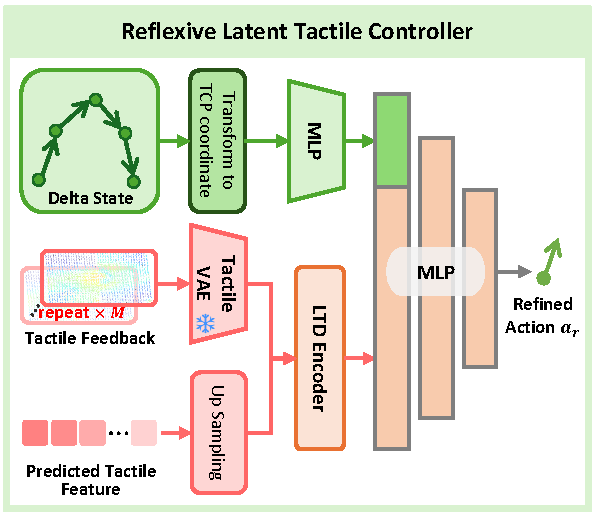
\includegraphics[width= 0.8\linewidth]{fig/controller.pdf}
\caption{\textbf{Overview of the Reflexive Latent Tactile Controller (RLTC).} It takes single-frame tactile feedback, predicted tactile latents, and robot/gripper delta states as input to produce high-frequency (60~Hz) refined single-step corrective actions.}
\label{fig:controller}
\end{figure}

\subsubsection{Training Loss}
To train the Reflexive Latent Tactile Controller, we learn corrective actions under abnormal contact conditions. For each task category, we first estimate a valid tactile distribution with its mean and standard deviation from human-collected trajectories. Tactile observations that fall outside this distribution (i.e., exhibiting excessively large or small contact forces) are identified as abnormal states.

We then extract recovery segments where the system transitions from abnormal tactile states back to the valid distribution, representing corrective behaviors demonstrated by human operators. 
For each time step in these segments, we construct training pairs consisting of the current tactile observation, the predicted tactile feature, and the corresponding corrective action $\hat{a}_r$.
The controller is trained to predict the corrective action $a_r$ using a mean squared error (MSE) loss:
\begin{equation}
\mathcal{L}_{RLTC} = \| a_r - \hat{a}_r \|_2^2,
\end{equation}
which encourages the controller to learn high-frequency tactile-driven corrections that stabilize contact interactions.
